\documentclass[11pt]{article}

\usepackage[review]{acl}
\usepackage{times}
\usepackage{latexsym}
\usepackage[T1]{fontenc}
\usepackage[utf8]{inputenc}
\usepackage{amsmath,amssymb}
\usepackage{booktabs}
\usepackage{graphicx}
\usepackage{microtype}
\usepackage{multirow}
\usepackage{tabularx}
\usepackage{xcolor}
\usepackage{inconsolata}
\usepackage{hyperref}
\usepackage{url}

\title{Decoding Schedules Reshape Repeated-Sampling Returns in Diffusion Language Models}

\author{Anonymous ACL submission}

\newcommand{\passk}{\operatorname{Pass@}k}
\newcommand{\cauc}{\operatorname{CoverageAUC}}
\newcommand{\model}{LLaDA-8B-Instruct}
\newcommand{\gsm}{GSM8K}
\newcommand{\mathfive}{MATH-500}
% Auto-generated by scripts/generate_manuscript_assets.py. Do not edit.
\newcommand{\OptionBPoint}{-0.044}
\newcommand{\OptionBLow}{-0.070}
\newcommand{\OptionBHigh}{-0.020}
\newcommand{\ConditionAPoint}{-0.010}
\newcommand{\ConditionALow}{-0.042}
\newcommand{\ConditionAHigh}{0.024}
\newcommand{\RandomPrimaryPoint}{+0.038}
\newcommand{\RandomPrimaryLow}{+0.003}
\newcommand{\RandomPrimaryHigh}{+0.074}
\newcommand{\BCIRho}{+0.014}
\newcommand{\BCIRhoLow}{-0.134}
\newcommand{\BCIRhoHigh}{+0.161}
\newcommand{\BCIMAE}{-0.000169}
\newcommand{\RandomNewPoint}{+0.038}
\newcommand{\RandomNewLow}{+0.005}
\newcommand{\RandomNewHigh}{+0.072}
\newcommand{\RandomSequentialLowPoint}{-0.033}
\newcommand{\RandomSequentialLowLow}{-0.052}
\newcommand{\RandomSequentialLowHigh}{-0.015}
\newcommand{\RandomSequentialFullPoint}{-0.018}
\newcommand{\RandomSequentialFullLow}{-0.039}
\newcommand{\RandomSequentialFullHigh}{+0.001}
\newcommand{\BlockLowGridPoint}{-0.020}
\newcommand{\BlockLowGridLow}{-0.040}
\newcommand{\BlockLowGridHigh}{+0.000}
\newcommand{\BlockHighGridPoint}{-0.047}
\newcommand{\BlockHighGridLow}{-0.079}
\newcommand{\BlockHighGridHigh}{-0.016}

% Auto-generated by scripts/generate_manuscript_assets.py. Do not edit.
\newcommand{\PostreviewMajorityVoteRows}{%
Sequential ($B=1$) & 0.535 & 0.545 & 0.565 & 0.608 & 0.610 & 0.618 & 0.630 \\
CF ($B=32$) & 0.550 & 0.542 & 0.585 & 0.587 & 0.585 & 0.585 & 0.585 \\
RND ($B=32$) & 0.460 & 0.468 & 0.539 & 0.589 & 0.589 & 0.612 & 0.611 \\
EF ($B=32$) & 0.355 & 0.380 & 0.480 & 0.536 & 0.558 & 0.579 & 0.575 \\
}

% Auto-generated by scripts/generate_manuscript_assets.py. Do not edit.
\newcommand{\GenerationAccountingRows}{%
Phase-0 signal & 3,200 \\
Phase-1 calibration & 6,400 \\
Held-out screening & 16,000 \\
Primary extension & 19,200 \\
Block-size extension & 19,200 \\
Entropy-first intervention & 12,800 \\
Random-policy extension & 9,600 \\
Temperature extension & 38,400 \\
\textbf{Total} & \textbf{124,800} \\
}

% Auto-generated by scripts/generate_manuscript_assets.py. Do not edit.
\newcommand{\MathDifficultyRows}{%
1 & 10 & 0.998 & 1.000 & 0.995 & 0.987 \\
2 & 19 & 0.754 & 0.769 & 0.766 & 0.715 \\
3 & 20 & 0.716 & 0.704 & 0.681 & 0.683 \\
4 & 23 & 0.513 & 0.386 & 0.460 & 0.433 \\
5 & 28 & 0.458 & 0.412 & 0.443 & 0.356 \\
}

% Auto-generated from the audited temperature reports. Do not edit.
\newcommand{\TempNineLowPoint}{-0.171}
\newcommand{\TempNineLowLower}{-0.231}
\newcommand{\TempNineLowUpper}{-0.112}
\newcommand{\TempNineHighPoint}{+0.013}
\newcommand{\TempNineHighLower}{-0.047}
\newcommand{\TempNineHighUpper}{+0.073}
\newcommand{\TempTwelveLowPoint}{-0.457}
\newcommand{\TempTwelveLowLower}{-0.516}
\newcommand{\TempTwelveLowUpper}{-0.397}
\newcommand{\TempTwelveHighPoint}{-0.196}
\newcommand{\TempTwelveHighLower}{-0.256}
\newcommand{\TempTwelveHighUpper}{-0.136}
\newcommand{\TempInteractionPoint}{-0.361}
\newcommand{\TempInteractionLower}{-0.402}
\newcommand{\TempInteractionUpper}{-0.321}
\newcommand{\TemperatureNewCount}{38,400}
\newcommand{\StudyGenerationCount}{124,800}
\newcommand{\TempCFEntropyBase}{0.238}
\newcommand{\TempCFEntropyMid}{0.238}
\newcommand{\TempCFEntropyHigh}{0.250}
\newcommand{\TempRandomGapBase}{0.208}
\newcommand{\TempRandomGapHigh}{0.377}
\newcommand{\TemperaturePrimaryRows}{%
0.9 & $-0.171$ & $[-0.231,-0.112]$ & $+0.013$ & $[-0.047,+0.073]$ \\
1.2 & $-0.457$ & $[-0.516,-0.397]$ & $-0.196$ & $[-0.256,-0.136]$ \\
}
\newcommand{\TemperatureDiagnosticRows}{%
0.6 & CF & 0.563 & 0.790 & 0.585 & 136.3 & 5.14 \\
0.6 & RND & 0.468 & 0.820 & 0.613 & 130.9 & 10.23 \\
0.6 & Sequential & 0.544 & 0.850 & 0.618 & 135.2 & 7.47 \\
0.9 & CF & 0.556 & 0.815 & 0.613 & 136.6 & 5.85 \\
0.9 & RND & 0.385 & 0.830 & 0.615 & 127.4 & 13.96 \\
0.9 & Sequential & 0.505 & 0.835 & 0.634 & 132.2 & 9.85 \\
1.2 & CF & 0.557 & 0.800 & 0.613 & 136.6 & 6.25 \\
1.2 & RND & 0.100 & 0.635 & 0.258 & 92.4 & 18.66 \\
1.2 & Sequential & 0.212 & 0.720 & 0.434 & 94.8 & 15.69 \\
}
\newcommand{\TemperatureTraceRows}{%
CF & 0.238 & 1.267 & 0.238 & 1.254 & 0.250 & 1.263 \\
RND & 0.411 & 0.407 & 0.662 & 0.667 & 3.580 & 3.584 \\
Sequential & 0.277 & 0.277 & 0.378 & 0.378 & 3.117 & 3.117 \\
}


\begin{document}

\maketitle

\begin{abstract}
Prior work reports that arbitrary-order decoding can lower the repeated-sampling coverage of masked diffusion language models. We test how robust this effect is, and where it stops, in a prospectively frozen, compute-matched design. Every schedule uses 256 neural function evaluations and commits one token after each; the block parameter $B$ changes only which positions are eligible. On one model and two mathematical-reasoning tasks, confidence-first $B=32$ minus sequential $B=1$ in mean Pass@$k$ over $k\in\{4,8,16,32,64\}$ is $\OptionBPoint$ (95\% CI $[\OptionBLow,\OptionBHigh]$), with no resolved loss at $k=1$; the effect is concentrated in the first widening and in a minority of queries. A targeted extension finds a small high-budget advantage of random over confidence-first ranking at temperature $0.6$ ($\RandomPrimaryPoint$, 95\% CI $[\RandomPrimaryLow,\RandomPrimaryHigh]$). It changes a pairwise ranking, while sequential decoding retains the highest high-budget point estimates. It is unresolved at $T=0.9$ ($\TempNineHighPoint$, $[\TempNineHighLower,\TempNineHighUpper]$) and reverses at $T=1.2$ ($\TempTwelveHighPoint$, $[\TempTwelveHighLower,\TempTwelveHighUpper]$). We show that aggregate Pass@$k$ crossings require heterogeneous per-query success differences, and that confidence-first couples position choice with candidate-token filtering, so low-entropy-position explanations are incomplete. Conclusions are limited to one model, two tasks, fixed compute, and oracle coverage.
\end{abstract}

\section{Introduction}

Masked diffusion language models (dLLMs) generate by repeatedly predicting masked tokens and choosing positions to commit. Unlike autoregressive language models, they need not use a fixed left-to-right order. This freedom can support genuinely parallel samplers, but it also changes the stochastic process that produces a solution even when the number of neural function evaluations (NFEs) is held fixed. Recent work has shown that arbitrary-order decoding can bypass uncertain ``forking'' positions and collapse solution coverage: arbitrary order can match or exceed left-to-right decoding at $k=1$ yet lose Pass@$k$ at large $k$, and block size, temperature, and random orders also shape these curves~\citep{ni2026flexibility}. We do not claim these phenomena as new. What remains open is how far they can be trusted and generalized: \emph{which of them survive a compute-matched, prospectively frozen test with query-level uncertainty, where do their boundaries lie in budget, temperature, and ranking rule, and which mechanistic explanations does the evidence actually support?}

The distinction matters because one-shot accuracy and repeated-sampling coverage answer different questions. A concentrated policy can be attractive when only one completion is available, while a policy that explores different solution basins can discover more correct answers as the sampling budget grows. Test-time scaling work routinely reports performance at several values of $k$~\citep{brown2024monkeys,snell2025scaling}, yet decoder comparisons are often compressed to one accuracy or an average over a chosen $k$-grid. Such compression can obscure the decision whenever the policy ranking changes over the deployment-relevant range.

We isolate two scheduling axes in a frozen model and evaluation pipeline: the eligible-set block size $B$, which ranges from a singleton left-to-right choice to a wider active block, and the position rule, which selects the next token by confidence, at random, or by predictive entropy. Importantly, every condition still commits one token per NFE; this is an NFE-matched study of order freedom, not a throughput study of simultaneous token commitment. Figure~\ref{fig:overview} previews the distinction. We evaluate \model{} on two mathematical-reasoning datasets using repeated rollouts, query-level inference, and an explicit evidence ledger separating prospectively frozen studies from analyses selected after unblinding.

\begin{figure*}[t]
  \centering
  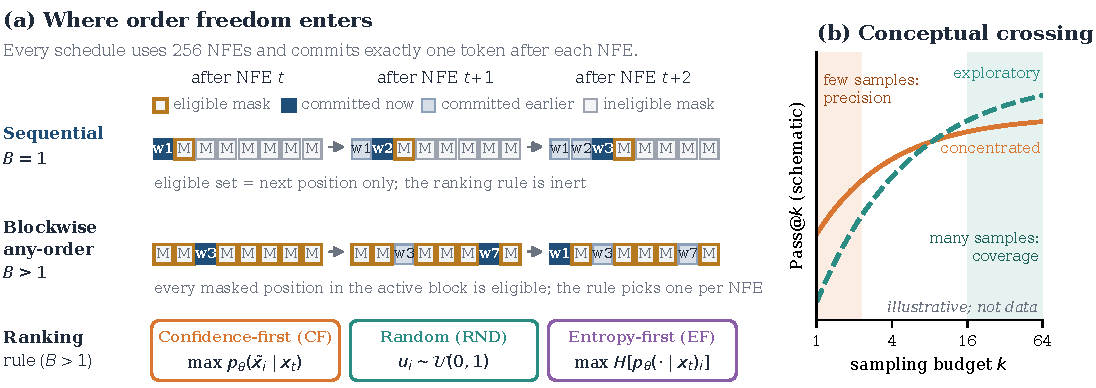
\includegraphics[width=\linewidth]{figures/fig1_overview.pdf}
  \caption{The decision studied in this paper. (a) Three successive NFEs of the evaluated implementation, which commits exactly one token per NFE under every schedule. At $B=1$ the only eligible position is the next one, so the ranking rule is inert; at $B>1$ every masked position in the active block is eligible, and the ranking rule (CF, RND, or EF) chooses which one to commit, together with its sampled candidate. (b) A conceptual sketch of an aggregate crossing; it contains no data (empirical frontiers: Figures~\ref{fig:frontier} and~\ref{fig:temperature}). Section~\ref{sec:estimand} shows that such crossings require success differences of opposite sign across queries.}
  \label{fig:overview}
\end{figure*}

Our contributions are three:
\begin{itemize}
  \item \textbf{A controlled test of the width effect.} Under 256 matched NFEs and one committed token per step, widening the eligible set from $B=1$ to $B=32$ under the confidence-first decoder lowers multi-sample coverage on both tasks without a resolved loss at $k=1$. The resolved change is confined to the first tested widening ($B=1\rightarrow8$; $B=2,4$ were not measured) and to a minority of queries.
  \item \textbf{Boundaries of the random-ranking effect.} A targeted extension finds a small, panel-level high-budget advantage of random over confidence-first ranking at $T=0.6$. It changes a pairwise ranking rather than the best tested policy, is unresolved at $T=0.9$, and reverses at $T=1.2$.
  \item \textbf{What the evidence can and cannot explain.} An aggregate Pass@$k$ crossing requires queries whose success differences have opposite signs, so it cannot by itself identify a per-query diversity benefit (Section~\ref{sec:estimand}). Confidence-first also couples position choice with candidate-token filtering (Section~\ref{sec:setup}), and entropy-first selection raises answer diversity without improving coverage.
\end{itemize}
The frozen protocols and evidence ledger (Section~\ref{sec:design}) support the credibility of these results; they are not themselves the contribution.

\section{Decoding Schedules and Estimands}
\label{sec:setup}

\subsection{Commitment schedules}

Let $x_t\in(\mathcal{V}\cup\{[\mathrm{MASK}]\})^L$ denote a partially masked sequence. At denoising step $t$, the model gives a categorical distribution $p_\theta(\cdot\mid x_t)$ for each masked position. A decoder samples candidate tokens and commits a subset of eligible positions; the remaining positions stay masked for a later step. This separates two choices.

\paragraph{Block size.}
The block size $B$ controls the scope from which the \emph{next} position may be selected. With generation length and denoising steps both fixed to 256, the implementation creates $256/B$ blocks and assigns $B$ denoising steps to each block. A block initially contains $B$ masks, so exactly one token is transferred at each step for every tested $B$. At $B=1$, the eligible set is a singleton and the same dLLM commits strictly left to right. For $B>1$, the policy selects one position from multiple masks in the active block. Thus $B$ varies eligible-set width and order freedom while holding NFEs and transfers per NFE fixed; it does not instantiate simultaneous multi-token commitment.

\paragraph{Position ranking.}
At each NFE the decoder draws one candidate token $\tilde x_i$ for every eligible position by Gumbel-max sampling at temperature $T$, scores the eligible positions, and commits the top-scoring position \emph{with its own candidate}. Within $B=32$ blocks we compare three scores: \textbf{confidence-first (CF)}, the untempered probability $p_\theta(\tilde x_i\mid x_t)$ of the position's own candidate; \textbf{random (RND)}, a uniform random score; and \textbf{entropy-first (EF)}, the entropy of the untempered distribution. EF is not the algebraic inverse of CF because the rules rank different quantities. Because CF scores each position by its own sampled candidate, it couples two choices: where to commit and which token to commit. If all eligible positions shared the distribution $P(a)=0.9$, $P(b)=0.1$, so that no position were more certain than another, CF at $T=1$ would still commit $a$ with probability $1-0.1^{B}$ rather than $0.9$. Widening the eligible set therefore also concentrates the committed tokens, independently of any difference in position entropy. We call the $B=1$ condition \textbf{sequential} rather than autoregressive: the underlying model remains the same dLLM. For artifact compatibility, the released code retains the historical key \texttt{ao} for CF.

\subsection{Coverage under repeated sampling}

For a query with $n$ sampled completions, of which $c$ are correct, we use the unbiased estimator introduced for repeated-sampling evaluation~\citep{chen2021codex}:
\begin{equation}
  \widehat{\operatorname{Pass@}k}
  = 1-\frac{\binom{n-c}{k}}{\binom{n}{k}}.
  \label{eq:passk}
\end{equation}
It estimates the probability that at least one of $k$ samples is correct. It is an \emph{oracle coverage} measure: deployment gains require a verifier or reranker that can identify a correct candidate. It should not be confused with majority-vote accuracy or single-sample precision.

For a declared grid $\mathcal{K}$, we define
\begin{equation}
  \cauc_{\mathcal{K}}(q,p)=\frac{1}{|\mathcal{K}|}\sum_{k\in\mathcal{K}}\widehat{\operatorname{Pass@}k}(q,p).
  \label{eq:cauc}
\end{equation}
Despite its name, $\cauc$ is a discrete, equally weighted mean over the declared grid, not an area under a continuous curve. Our block-size primary uses $\mathcal{K}_{64}=\{4,8,16,32,64\}$. We always name the grid because a coverage average implicitly specifies a distribution over sampling budgets. With $n=k=64$, Eq.~\eqref{eq:passk} reduces to the indicator that at least one of the 64 rollouts is correct.

\section{Experimental Design and Evidence Status}
\label{sec:design}

\paragraph{Model and tasks.}
We evaluate \model{}~\citep{nie2025llada}, revision \texttt{08b83a6}, with a traced reimplementation of the JustGRPO decoder~\citep{ni2026flexibility} at commit \texttt{1a2fddb}, whose public default is $B=32$ confidence remasking with one token per step; unlike the public code, we compute CF confidences in float32 rather than bfloat16. We use 100 held-out queries from \gsm{}~\citep{cobbe2021gsm8k} and 100 from \mathfive{}~\citep{hendrycks2021math}. The main and original follow-up conditions have 64 rollouts per query and generate 256 positions in 256 denoising steps at temperature $0.6$ and classifier-free-guidance scale $0$. The temperature extension adds 32 rollouts per query and cell at $T\in\{0.9,1.2\}$. All conditions use 256 NFEs and one committed token per NFE. GSM8K answers are extracted with the JustGRPO GSM8K parser and compared with its mathematical-equivalence checker; MATH-500 targets and predictions use the same repository's generic answer extractor and timeout-protected equivalence checker. Parser failures and empty responses are retained as incorrect. All primary intervals use a paired, task-stratified bootstrap over queries (10,000 replicates); rollouts and token events are never treated as independent samples.

\paragraph{Evidence ledger.}
The study evolved through falsifiable stages rather than one retrospective analysis. Table~\ref{tab:ledger} records both the selection history and the question frozen before each outcome read. Protocols fix model and data revisions, query IDs, seeds, endpoints, bootstrap rules, artifact cardinalities, and decision criteria. Across the formal and signal stages, we evaluated \StudyGenerationCount{} generations, excluding smoke and replay checks.

\begin{table}[t]
\caption{Evidence ledger. Selection history is explicit because targeted prospective studies were chosen after earlier results but frozen before their new outcomes were read. The final column records evidentiary role, not statistical outcome.}
\label{tab:ledger}
\centering
\scriptsize
\setlength{\tabcolsep}{2pt}
\begin{tabular}{@{}>{\raggedright\arraybackslash}p{0.9cm}>{\raggedright\arraybackslash}p{1.45cm}>{\raggedright\arraybackslash}p{2.35cm}>{\raggedright\arraybackslash}p{1.65cm}@{}}
\toprule
Study & Selection history & Frozen question & Evidentiary role \\
\midrule
Block size & Prospective before outcomes & $B=32$ vs. $B=1$; trend & Primary confirmatory \\
EF test & Prospective; gated & EF vs. CF $\cauc_{\mathcal K_{64}}$ & Prospective intervention \\
Random ext. & After first-16 crossing; frozen before new outcomes & Mean RND--CF at $k=16,32,64$ & Scoped prospective follow-up \\
Temp. ext. & After review; frozen before new outcomes & RND--CF reversal at $T=0.9,1.2$ & Scoped prospective follow-up \\
Audits & Post-outcome & Per-$k$, multiplicity, diversity, traces & Exploratory/\newline secondary \\
\bottomrule
\end{tabular}
\end{table}

\section{Widening the Eligible Set Lowers Repeated-Sampling Coverage}
\label{sec:block}

We first estimate the total effect of widening the eligible set under the confidence-first decoder, varying $B\in\{1,8,16,32\}$ while holding the model, queries, rollout budget, 256 NFEs, one transfer per NFE, and all other decoding settings fixed. This total effect bundles order freedom with CF's candidate filtering (Section~\ref{sec:setup}); the design does not separate them. The prospectively frozen primary contrast is
$\cauc_{\mathcal K_{64}}(B=32)-\cauc_{\mathcal K_{64}}(B=1)$.
It is $\OptionBPoint$ with 95\% CI $[\OptionBLow,\OptionBHigh]$; the interval is below zero both on \gsm{} and \mathfive{}. Meanwhile the pooled Pass@1 point estimate rises from $\BlockPassOneSequential$ to $\BlockPassOneWide$, while Pass@16 falls from $\BlockPassSixteenSequential$ to $\BlockPassSixteenWide$. A single-sample comparison would therefore miss the principal change in repeated-sampling returns.

\begin{figure}[t]
  \centering
  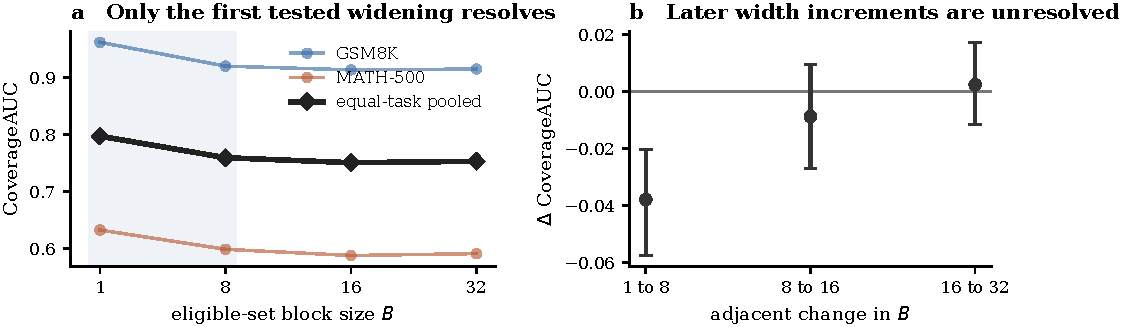
\includegraphics[width=\linewidth]{figures/fig2_block_size.pdf}
  \caption{\textbf{Only the first tested eligible-set widening gives a resolved adjacent contrast.} (a) Change in $\cauc_{\{4,8,16,32,64\}}$ relative to $B=1$ on a $\log_2 B$ axis. The hatched region marks the unmeasured $B=2,4$; dotted segments cross it without implying a shape. Error bars at the right are the frozen $B=32-B=1$ intervals. (b) Paired adjacent pooled contrasts with pointwise 95\% query-bootstrap intervals. The $1\rightarrow8$ decrease resolves; the later adjacent changes do not. All settings use 256 NFEs and commit one token per NFE.}
  \label{fig:block}
\end{figure}

Figure~\ref{fig:block} qualifies the second frozen endpoint, a slope on $\log_2 B$. That slope also resolves below zero ($\OptionBTrendPoint$ per doubling; 95\% CI $[\OptionBTrendLow,\OptionBTrendHigh]$), but an exact decomposition attributes \BlockTrendStepShare{} of its magnitude to the step from $B=1$ to the block-parallel settings. Correspondingly, the $B=1\rightarrow8$ contrast is $\BlockStepOneEightPoint$ $[\BlockStepOneEightLow,\BlockStepOneEightHigh]$, whereas $8\rightarrow16$ and $16\rightarrow32$ both straddle zero, and the two frozen query-level endpoints are highly dependent (Pearson $r=\BlockEndpointPearson$; tie-aware Spearman $\rho=\BlockEndpointSpearman$). We therefore interpret the evidence as one resolved singleton-to-wider-set contrast on a coarse grid, not as multiple independent confirmations, a smooth law over $B$, an identified threshold location, or an effect of reducing NFEs.

The effect also depends on sampling budget. A post-outcome grid audit estimates $B=32-B=1$ as $\BlockLowGridPoint$ $[\BlockLowGridLow,\BlockLowGridHigh]$ on $k\in\{1,2,4,8\}$, which does not strictly exclude zero, and $\BlockHighGridPoint$ $[\BlockHighGridLow,\BlockHighGridHigh]$ on $k\in\{16,32,64\}$. Per-$k$ contrasts are near zero at $k=1,2$ and resolve below zero from $k=4$ onward (Appendix~\ref{app:postreview}). Thus the primary finding concerns repeated-sampling coverage; it is not a claim that a wider eligible set uniformly harms every budget.

An exploratory query-level audit shows that the pooled effect is concentrated in a minority of queries rather than carried by a single one. The median query effect is zero, \FragilitySmallEffectCount{} of 200 queries change by less than $0.01$, and the ten most-hurt queries carry \FragilityTopTenShare{} of the summed effect. No single query is decisive (the largest leave-one-query-out change is $0.0039$), but removing the \FragilityRemovedForZero{} most-hurt queries brings the interval to zero. This outcome-selected removal describes concentration rather than testing the effect, and it is why replication on new queries or models matters more than further reanalysis of this panel.

\section{Sampling Budget Changes a Pairwise Policy Ranking}
\label{sec:policies}

We next hold $B=32$ fixed and vary the position-ranking rule. The original RND condition had only 16 rollouts. After an exploratory analysis suggested a crossing with CF, we froze a targeted extension before generating 48 additional RND rollouts for every held-out query. The final estimator combines these 48 new and 16 previously observed rollouts; it is prospective only with respect to the new outcomes and lies outside the original confirmatory chain.

\begin{figure}[t]
  \centering
  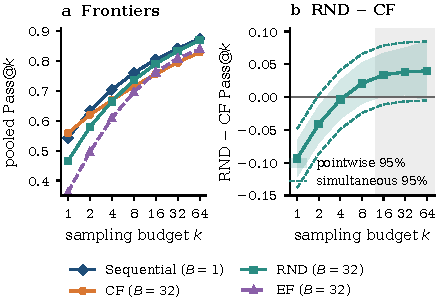
\includegraphics[width=\linewidth]{figures/fig3_policy_frontier.pdf}
  \caption{\textbf{Position ranking reshapes the sampling-budget frontier.} (a) Equal-task pooled $\passk$ for four schedules at $T=0.6$ (64 rollouts per query). (b) Paired RND minus CF with pointwise (shaded) and seven-endpoint simultaneous (dashed) 95\% query-bootstrap bands from the post-outcome multiplicity audit (Appendix~\ref{app:multiplicity}). CF is favored at small $k$ and the contrast changes sign as $k$ grows, but no positive per-$k$ point survives the simultaneous band; the frozen evidence is the single high-budget mean over the gray region.}
  \label{fig:frontier}
\end{figure}

The frozen high-budget functional averages the paired RND--CF difference at $k\in\{16,32,64\}$. Its pooled value is $\RandomPrimaryPoint$ (95\% CI $[\RandomPrimaryLow,\RandomPrimaryHigh]$). Task-specific estimates are similar in sign and magnitude but each interval crosses zero, so the claim is panel-level rather than replicated separately by task. At low budget, the exploratory pointwise RND--CF estimates have the opposite sign: $-0.094$ at $k=1$ and $-0.041$ at $k=2$. Taken together, these estimates support a scoped budget interaction, not universal RND superiority or a claim that random ranking is the best policy.

Because the final 64-rollout estimator includes the 16 rollouts that motivated the extension, we also ran a post-outcome independence audit restricted to the 48 outcomes that were unseen when the extension was frozen. Over its feasible high-budget grid $k\in\{16,32\}$, RND--CF is $\RandomNewPoint$ $[\RandomNewLow,\RandomNewHigh]$; the individual $k=16$ and $k=32$ intervals also exclude zero. The old-16 minus new-48 RND curve straddles zero at every comparable $k$ (Appendix~\ref{app:postreview}). This audit does not upgrade the study to independent preregistered replication, but it shows that the crossing is not carried by the outcome-selected first 16 rollouts.

Sequential $B=1$ retains slightly higher high-budget point estimates than RND, but the paired RND--sequential intervals include zero at each of $k=16,32,64$. Conversely, CF has the highest Pass@1 point estimate among the tested $B=32$ policies. The crossing is therefore a budget-dependent change in the CF--RND ranking, not evidence of a switch in the best tested policy. These are equal-rollout, equal-NFE comparisons, not latency-controlled utility frontiers: a practical decoder choice must jointly price wall-clock cost, sampling budget, and verifier quality.

The available paired RND--sequential contrast helps, but does not fully separate, width from ranking. It is $\RandomSequentialLowPoint$ (95\% CI $[\RandomSequentialLowLow,\RandomSequentialLowHigh]$) over $k\in\{2,4,8,16\}$, favoring sequential at low budget, but $\RandomSequentialFullPoint$ (95\% CI $[\RandomSequentialFullLow,\RandomSequentialFullHigh]$) over $k\in\{4,8,16,32,64\}$. Thus the data support a scoped low-budget sequential advantage over random selection, while the ranking component remains unresolved on the full high-budget grid.

A descriptive, tie-aware majority-vote analysis does not turn oracle coverage into a deployment result, but it provides a useful check. At $k=1$, pooled majority-vote accuracy is $0.550$ for CF and $0.460$ for RND; the paired unadjusted query-bootstrap intervals for both Sequential--RND ($+0.075$ $[+0.005,+0.140]$) and CF--RND ($+0.090$ $[+0.030,+0.155]$) exclude zero. At $k=16,32,64$, both comparisons include zero. These statistics use the first $k$ rollout indices rather than averaging over $k$-subsets, so MV@1 need not equal the subset-averaged Pass@1; they are post-outcome and not multiplicity-adjusted, so we report the full curves in Appendix~\ref{app:postreview} rather than treating them as a new confirmatory endpoint.

\subsection{Maximizing answer diversity is not sufficient}

The prospectively frozen EF intervention does not improve the aggregate endpoint over CF: EF--CF is $\ConditionAPoint$ with 95\% CI $[\ConditionALow,\ConditionAHigh]$. The interval crossing zero is unresolved, not evidence of equivalence. A preregistered guard also finds that EF responses are shorter by 9.83 whitespace tokens on average, requiring this result to be interpreted with caution.

Nevertheless, the intervention clearly changes the output distribution. At $k=64$, EF has parsed-answer entropy $1.90/2.48$ on \gsm{}/\mathfive{}, versus $1.18/2.10$ for random; yet random exceeds EF in correct coverage over most measured budgets. Figure~\ref{fig:diversity} shows the separation. Parsed-answer entropy measures answer strings, not semantic reasoning paths. This descriptive pattern, four policy points without intervals, is inconsistent with treating answer diversity as a sufficient proxy for correct coverage; it does not test whether diversity helps in general.

\begin{figure}[t]
  \centering
  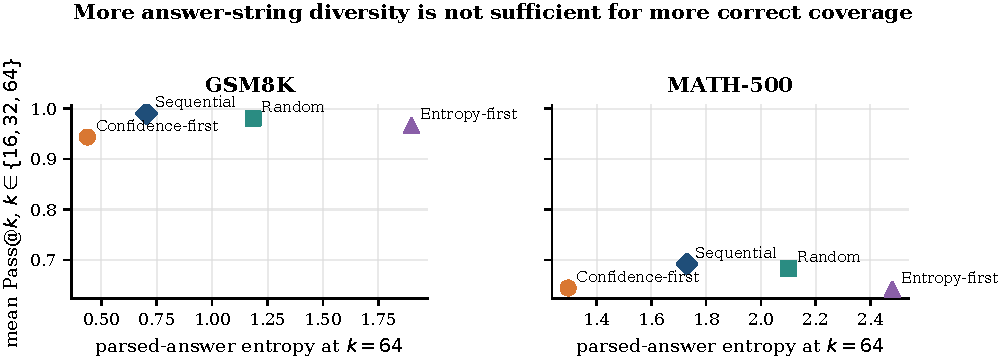
\includegraphics[width=\linewidth]{figures/fig4_diversity.pdf}
  \caption{\textbf{More parsed-answer diversity is not sufficient for greater correct-answer coverage.} Each point is a policy at $k=64$; the vertical axis averages Pass@$k$ over $k\in\{16,32,64\}$. EF has higher parsed-answer entropy than RND on both tasks without occupying a uniformly higher-coverage region. Descriptive only: no intervals, and the vertical axes are truncated and differ by task.}
  \label{fig:diversity}
\end{figure}

\section{Temperature Changes the Policy Frontier}
\label{sec:temperature}

The schedule comparison was then tested at two additional sampling temperatures, $T=0.9$ and $T=1.2$, using the same model, queries, 256 NFEs, and three schedules. This extension was selected after review of the earlier results and frozen before its 38,400 new generations were evaluated; it is a prospective follow-up outside the original Gate-1 chain. The frozen family tests whether the RND--CF contrast is below zero at $k=1$ and above zero at the mean of $k=16$ and $32$. Because each new cell has 32 rollouts, this high-budget functional stops at $k=32$; Table~\ref{tab:temperature-primary} therefore also lists the reused $T=0.6$ arm under the same functional as a descriptive reference.

\begin{table}[t]
\caption{Temperature-extension endpoints: RND minus CF at $k=1$ and at the mean of $k=16,32$. Intervals are simultaneous 95\% query-bootstrap bands over the four frozen endpoints. $^\dagger$Descriptive reference from the first 32 reused $T=0.6$ rollouts; not part of the frozen family.}
\label{tab:temperature-primary}
\centering
\small
\resizebox{\columnwidth}{!}{%
\begin{tabular}{c r@{\ }l r@{\ }l}
\toprule
$T$ & \multicolumn{2}{c}{RND--CF $k=1$} & \multicolumn{2}{c}{RND--CF high budget} \\
\midrule
\TemperaturePrimaryRows
\bottomrule
\end{tabular}%
}
\end{table}

The frozen verdict is ``not resolved as reversal'' at both temperatures. At $T=0.9$, the low-budget contrast is resolved below zero, but the high-budget estimate is $\TempNineHighPoint$ with an interval crossing zero; this is not evidence of equivalence, since no equivalence margin was specified. At $T=1.2$, the high-budget contrast is resolved in the opposite direction ($\TempTwelveHighPoint$, 95\% simultaneous CI $[\TempTwelveHighLower,\TempTwelveHighUpper]$). Within this model and task panel, the $T=0.6$ high-budget advantage of RND ($\TempSixHighPoint$ under this functional) is therefore temperature-conditional. Estimated directly on the shared window with 32 rollouts per cell, the post-hoc interaction $[\mathrm{RND}-\mathrm{CF}]_{T}-[\mathrm{RND}-\mathrm{CF}]_{0.6}$ is $\TempInteractionHighNinePoint$ ($[\TempInteractionHighNineLower,\TempInteractionHighNineUpper]$, unadjusted) at $T=0.9$ and $\TempInteractionHighTwelvePoint$ ($[\TempInteractionHighTwelveLower,\TempInteractionHighTwelveUpper]$) at $T=1.2$: the two temperatures differ in kind, one inconclusive and one a clear reversal. The sequential comparison also depends on temperature: its modest high-budget point advantage over CF at $T=0.6$ is absent at $T=1.2$.

\begin{figure}[t]
  \centering
  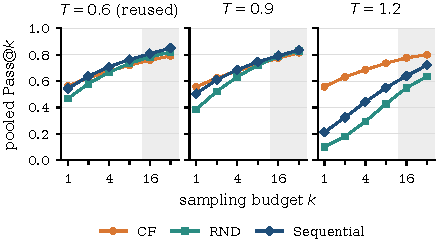
\includegraphics[width=\linewidth]{figures/fig5_temperature_frontier.pdf}
  \caption{\textbf{Temperature changes the policy frontier.} Equal-task pooled Pass@$k$ for the three schedules at the reused $T=0.6$ condition and the two new temperatures. The $T=0.9$ crossing is attenuated and unresolved under the frozen high-budget family; at $T=1.2$, random and sequential coverage fall while confidence-first remains comparatively stable. Gray: the frozen high-budget window $k\in\{16,32\}$.}
  \label{fig:temperature}
\end{figure}

The extension also reveals differential sensitivity. Relative to $T=0.6$, the exploratory paired change in random-minus-confidence Pass@1 is $\TempInteractionPoint$ at $T=1.2$ (unadjusted 95\% CI $[\TempInteractionLower,\TempInteractionUpper]$), while confidence-first itself changes by only $-0.006$ (CI $[-0.021,+0.010]$). These comparisons were selected after outcomes were read and are descriptive. Trace diagnostics are consistent with the explanation that confidence-first keeps committing positions with low model-distribution entropy: across all 200 queries and two rollouts per cell, selected-position entropy for CF is $\TempCFEntropyBase$, $\TempCFEntropyMid$, and $\TempCFEntropyHigh$ at $T=0.6,0.9,1.2$, far below the ${\approx}1.26$ mean entropy of its eligible positions, whereas it rises from $0.41$ to $3.58$ for RND and from $0.28$ to $3.12$ for sequential decoding (Appendix~\ref{app:temperature}). This pattern is expected when temperature perturbs candidate sampling but CF ranks positions by untempered probabilities. It is not a causal decomposition: each policy visits different states, and CF also filters the committed candidate (Section~\ref{sec:setup}), so trajectory averages cannot separate the selection rule from state evolution. The trace field called \texttt{candidate\_probabilities} stores random selection scores for RND and must not be interpreted as model probabilities across policies.

\section{What an Aggregate Crossing Can and Cannot Show}
\label{sec:estimand}

Let $s_\pi(q)$ be policy $\pi$'s single-sample success probability on query $q$. Under independent repeated sampling, expected coverage is $F_\pi(k)=\mathbb{E}_q\bigl[1-(1-s_\pi(q))^k\bigr]$.

\paragraph{Proposition.} If $s_\pi(q)\geq s_{\pi'}(q)$ for every query $q$, then $F_\pi(k)\geq F_{\pi'}(k)$ for every $k$. This follows because $1-(1-s)^k$ is nondecreasing in $s$ for each $k$; the unbiased estimator in Eq.~\eqref{eq:passk} is likewise nondecreasing in $c$ for fixed $n$ and $k$.

An aggregate crossing such as CF--RND in Figure~\ref{fig:frontier} therefore implies queries whose success differences have opposite signs, reweighted by budget. This is a necessary condition for interpreting a crossing, not a mechanism theorem. For two equally weighted queries with $s_{\mathrm{CF}}=(0.9,0.1)$ and $s_{\mathrm{RND}}=(0.6,0.25)$, CF has the higher Pass@1 ($0.500$ vs.\ $0.425$), yet at $k=8$ coverage is $0.785$ for CF and $0.950$ for RND. Diversity may still act by changing $s_\pi(q)$, but Pass@$k$ curves alone cannot identify that mechanism.

The same heterogeneity makes scalar summaries grid-dependent. Any weighted summary $\Delta_w=\sum_{k\in\mathcal K}w_k\Delta(k)$ with $w_k\geq0$ and $\sum_k w_k=1$ lets regions of opposite sign cancel. The frozen EF--CF $\cauc_{\mathcal K_{64}}$ contrast is unresolved, but the same 64 rollouts give $-0.050$ on $\{2,4,8,16\}$ and $+0.010$ on $\{16,32,64\}$ in a post-outcome decomposition. A weighting is appropriate when it represents a deployment distribution; otherwise the frontier should be reported. Finally, under seven-endpoint maximum-deviation bands, only the $k=1$ RND--CF point survives (Appendix~\ref{app:multiplicity}). The evidentiary anchor remains the separately frozen high-budget mean, which tests a different hypothesis from the pointwise family.

\section{Related Work}

\paragraph{From discrete diffusion to masked language models.}
Early discrete diffusion constructions define categorical corruption and denoising processes directly in token space~\citep{hoogeboom2021argmax,austin2021structured}; continuous Diffusion-LM instead denoises latent word vectors for controllable generation~\citep{li2022diffusionlm}. Subsequent work improves discrete objectives through ratio estimation~\citep{lou2024sedd} and simplifies the training objective and parameterization of absorbing-mask models~\citep{shi2024masked,ou2025absorbing}. Masked diffusion language models (MDLMs) then establish competitive text modeling and scaling behavior~\citep{sahoo2024mdlm,nie2025scaling}, while LLaDA extends masked diffusion to instruction following and mathematical reasoning at the scale used here~\citep{nie2025llada}. This lineage creates the distinctive decision studied in our paper: unlike left-to-right generation, an MDLM can choose \emph{which} position to reveal next, so inference order is part of the generative process rather than an implementation detail.

\paragraph{Unmasking order and schedule theory.}
Token order can affect both likelihood and the difficulty of intermediate infilling problems. Adaptive planning can avoid unfavorable orders~\citep{kim2025ordering}; learned reference policies and lookahead scores similarly optimize where to unmask~\citep{hong2025policies,asano2026where,lee2025lookahead}. Complementary theory bounds distributional error under masked-diffusion schedules and characterizes when parallel updates are valid~\citep{chen2026optimal}. The closest prior work is the Flexibility Trap~\citep{ni2026flexibility}. It shows that arbitrary-order decoding can bypass uncertain forking positions and lower large-$k$ Pass@$k$, examines block size, temperature, and random orders, and then proposes training dLLMs with GRPO in left-to-right order. We take its central phenomenon as given. Our contribution is a compute-matched, prospectively frozen test of it with query-level uncertainty, a necessary condition for interpreting aggregate crossings, and an analysis of what trajectory diagnostics can and cannot identify. Its random and entropy-based orders need not coincide with our settings: the public decoder at our pinned commit implements confidence and block-local random remasking only, and EF is our addition.

\paragraph{Parallel decoding and inference acceleration.}
A separate line of work exploits the same non-autoregressive structure for throughput. Fast-dLLM combines parallel commitment with cache reuse, and EB-Sampler uses an entropy constraint to commit multiple positions~\citep{wu2026fastdllm,benhamu2025ebsampler}. Adaptive Parallel Decoding uses an auxiliary autoregressive model to vary safe parallelism~\citep{israel2025apd}; AdaBlock-dLLM and Dynamic-dLLM instead adapt block boundaries, cache budgets, or commitment thresholds~\citep{lu2026adablock,wu2026dynamic}. These systems study a quality--latency frontier in which the number of tokens committed per NFE may change. Our intervention is intentionally orthogonal: every condition uses 256 NFEs and commits exactly one token after each. Consequently, our $B$ is an \emph{eligible-set width}, not a claim of wall-clock acceleration, and our results neither rank those accelerators nor establish an optimal schedule.

\paragraph{Test-time scaling and candidate selection.}
Repeated sampling can improve the probability of discovering a correct response without changing model parameters~\citep{brown2024monkeys}, while compute-optimal allocation depends on problem difficulty and the available selection mechanism~\citep{snell2025scaling}. Budget forcing provides another route to scaling reasoning-time compute within a trajectory~\citep{muennighoff2025s1}. Selection also changes the relevant estimand: self-consistency aggregates final answers~\citep{wang2023selfconsistency}, process reward models score intermediate reasoning steps~\citep{lightman2024verify}, and Pass@$k$ measures oracle discovery of at least one correct candidate~\citep{chen2021codex}. We deliberately use the last quantity to isolate candidate-set coverage, then report majority-vote results separately. Our findings therefore do not imply deployable gains without a verifier or reranker.

\paragraph{Sampling diversity and budget-dependent evaluation.}
Decoding has long been understood to trade concentration against diversity: maximization can produce degenerate text, whereas truncated stochastic sampling broadens the support while controlling low-probability tails~\citep{holtzman2020degeneration}. In reasoning, however, more surface-form diversity need not mean more \emph{correct} solution coverage. Our entropy-first result makes that distinction explicit, while the CF--RND crossing adds an evaluation issue not captured by a single diversity statistic. If policy contrasts change sign with $k$, averaging Pass@$k$ over several budgets can attenuate the difference by construction. The resulting scalar is meaningful only relative to its declared weights; otherwise, the deployment-relevant object is the budget-indexed frontier.

\section{Discussion}

The experiments provide a decision map over measured estimands rather than one universally best policy. At $k=1$, CF has the highest measured point estimate among the $B=32$ policies, and its exploratory coverage point estimate remains higher at $k=2$; against sequential decoding, its Pass@1 advantage is unresolved ($+0.016$ $[-0.005,+0.037]$). On the frozen pooled high-budget functional at $T=0.6$, RND recovers part of CF's coverage loss, while sequential commitment retains slightly higher point estimates. Under descriptive majority voting, sequential decoding has the highest point estimate among the four policies in Table~\ref{tab:majority} at every $k\geq8$; this makes it the strongest point-estimate baseline in that table, not a statistically established dominance claim. Entropy-first may be useful as a candidate generator only if a downstream selector can exploit its extra diversity; our oracle-coverage results do not demonstrate such a selector.

The resolved $B=1\rightarrow8$ contrast admits two routes that the design does not separate. Once $B>1$, the committed position can depend on sampled model state; in addition, CF selects among $B$ sampled candidates, which concentrates the committed tokens even without differences in position entropy (Section~\ref{sec:setup}). A control that keeps CF's position choice but redraws the committed token from the same tempered distribution would separate the two at no extra NFE cost. The unmeasured $B=2,4$ settings leave gradual change within $[1,8]$ equally compatible with the data. A separately frozen local uncertainty index also failed its held-out targeting test (Appendix~\ref{app:bci}).

\section{Conclusion}

In the tested dLLM, widening the next-position eligible set under confidence-first decoding lowers repeated-sampling coverage without a resolved loss at $k=1$, consistent with prior reports; under a frozen, compute-matched design the effect is concentrated in the first widening and in a minority of queries. The high-budget advantage of random ranking at $T=0.6$ changes a pairwise ranking, is unresolved at $T=0.9$, and reverses at $T=1.2$, while sequential decoding remains the strongest tested baseline. Aggregate crossings reflect heterogeneity across queries, and CF couples position choice with token filtering, so neither the curves nor trajectory entropies identify a diversity mechanism. Report the frontier, or state the weighting used to compress it.

\section{Limitations}
\label{sec:limitations}

The study uses one frozen model checkpoint, two mathematical-reasoning datasets with 100 held-out queries each, three tested temperatures, a fixed sequence length, and one implementation of each policy; task-specific intervals are therefore wide, the random-extension claim is panel-level only, and the block-size effect is concentrated in fewer than 20 of the 200 queries. The random and temperature extensions were selected after earlier evidence or review and combine targeted follow-up designs with the original study; their selection histories remain visible in Table~\ref{tab:ledger}. The temperature extension has 32 rollouts per cell, so its high-budget functional is not identical to the 64-rollout functional at $T=0.6$. No equivalence margins were prespecified, so unresolved contrasts are not evidence of equivalence. Per-$k$ multiplicity, post-treatment response length, task ceilings, and an oracle correctness grader all constrain interpretation. The temperature trace diagnostic is based on two rollout traces per query and does not identify a causal mechanism. Most importantly, coverage is not realized utility without a verifier, and we do not report a controlled quality--latency--memory frontier. The random-ranking effect has not been validated on unseen problems, and CF's position selection has not been separated from its candidate filtering. Cross-model, non-mathematical, and verifier-based tests are therefore questions for future work rather than claims of this paper.

\section*{AI Use Statement}

During research and manuscript preparation, the authors used OpenAI Codex and Anthropic Claude to assist with manuscript drafting and revision, reference formatting and checking, experimental-protocol development, code implementation and debugging, figure generation, and statistical analysis. The authors made the final research decisions, supervised computational execution, and reviewed and verified the AI-assisted outputs, including reported results and interpretations. The authors take full responsibility for the paper.

\bibliography{references}

\appendix

\section{Frozen Experimental Configuration}
\label{app:protocol}

Table~\ref{tab:config} records the configuration shared by all held-out interventions. Dataset rows, prompts, and split roles were pinned by hash before inference. The same query/rollout seed key was assigned across policies, although diverging trajectories consume random draws differently and therefore do not constitute stepwise common random numbers.

\begin{table}[h]
\caption{Frozen held-out configuration.}
\label{tab:config}
\centering
\small
\begin{tabular}{@{}p{2.0cm}p{4.9cm}@{}}
\toprule
Item & Value \\
\midrule
Model & \texttt{GSAI-ML/LLaDA-8B-Instruct} \\
Model revision & \texttt{08b83a6f}\allowbreak\texttt{eb34df1a}\allowbreak\texttt{6011b80c}\allowbreak\texttt{3c00c756}\allowbreak\texttt{3e963b07} \\
Decoder & reimplementation of \url{LeapLabTHU/JustGRPO}, commit \texttt{1a2fddb5}; CF confidence in float32 \\
Tasks & 100 held-out \gsm{} + 100 held-out \mathfive{} queries \\
Decoding & 256 positions, 256 denoising steps \\
Sampling & main: $T=0.6$; extension: $T\in\{0.9,1.2\}$; CFG scale 0 \\
Inference unit & query; paired, task-stratified bootstrap \\
Bootstrap & 10,000 replicates, percentile 95\% interval \\
\bottomrule
\end{tabular}
\end{table}

\section{Block-Size Results}

\begin{table}[h]
\caption{Absolute $\cauc_{\{4,8,16,32,64\}}$ by block size.}
\centering
\begin{tabular}{rrrr}
\toprule
$B$ & Pooled & \gsm{} & \mathfive{} \\
\midrule
1  & 0.79746 & 0.96236 & 0.63256 \\
8  & 0.75960 & 0.92045 & 0.59874 \\
16 & 0.75084 & 0.91390 & 0.58778 \\
32 & 0.75325 & 0.91534 & 0.59115 \\
\bottomrule
\end{tabular}
\end{table}

The first Option-B analysis invocation terminated before emitting an endpoint because valid all-zero cells had not been materialized in the analyzer's expected-cell map. The repair explicitly initializes every expected cell, was bound by a pre-analysis amendment, and was rerun from the raw artifacts; no pre-repair endpoint entered a gate or interpretation. The repaired analyzer independently reproduced the primary point estimate to numerical precision. All 51,200 expected records validated; 132 of 800 query--task--block cells had zero successes and were retained.

\section{RND--CF Multiplicity Audit}
\label{app:multiplicity}

\begin{table}[h]
\caption{RND minus CF per-$k$ contrasts from a post-outcome audit with 50,000 task-stratified paired-query bootstrap replicates. Raw intervals are unadjusted and can differ in the third decimal from the frozen analyzer's 10,000-replicate secondary intervals; simultaneous intervals use a seven-endpoint nonstudentized maximum-deviation family.}
\centering
\small
\resizebox{\columnwidth}{!}{%
\begin{tabular}{r r@{ }l r@{ }l}
\toprule
$k$ & \multicolumn{2}{c}{Raw 95\% CI} & \multicolumn{2}{c}{Simultaneous 95\% CI} \\
\midrule
1  & $-0.094$ & [$-0.121,-0.067$] & $-0.094$ & [$-0.139,-0.049$] \\
2  & $-0.041$ & [$-0.070,-0.014$] & $-0.041$ & [$-0.086,+0.004$] \\
4  & $-0.004$ & [$-0.033,+0.026$] & $-0.004$ & [$-0.049,+0.041$] \\
8  & $+0.021$ & [$-0.010,+0.053$] & $+0.021$ & [$-0.024,+0.066$] \\
16 & $+0.034$ & [$+0.002,+0.067$] & $+0.034$ & [$-0.011,+0.079$] \\
32 & $+0.038$ & [$+0.003,+0.075$] & $+0.038$ & [$-0.007,+0.083$] \\
64 & $+0.040$ & [$-0.005,+0.085$] & $+0.040$ & [$-0.005,+0.085$] \\
\bottomrule
\end{tabular}%
}
\end{table}

The post-outcome two-region diagnostic averages $k=1,2$ and $k=16,32$. Its two-endpoint simultaneous intervals are $-0.067$ $[-0.102,-0.032]$ and $+0.036$ $[+0.001,+0.071]$, respectively. This reduced family diagnoses the crossing but cannot replace the frozen high-budget endpoint.

\section{Post-Review Independence and Robustness Audits}
\label{app:postreview}

All analyses in this section were specified after the 64-rollout RND extension was unblinded. They are exploratory diagnostics and do not alter any frozen endpoint or verdict. Restricting RND and CF to matched rollout indices 16--63 gives RND--CF contrasts of $+0.0358$ $[+0.0027,+0.0694]$ at $k=16$ and $+0.0399$ $[+0.0045,+0.0769]$ at $k=32$. Their prespecified-for-this-audit mean is \RandomNewPoint{} $[\RandomNewLow{},\RandomNewHigh{}]$. Comparisons of the first 16 RND rollouts with the later 48 give intervals spanning zero for every $k\leq16$. A split-half check preserves the negative low-budget direction in both halves; positive high-budget estimates are clearer in the second half. Together these diagnostics support exchangeability of the added rollouts while retaining the extension's targeted, post-unblinding-selected status.

Table~\ref{tab:majority} reports a deployment-adjacent secondary metric. We group identical nonempty parsed answers, select the modal answer, and average correctness uniformly across tied modes. Values use the first $k$ frozen rollout indices, so they are descriptive prefix estimates rather than subset-averaged estimators.

\begin{table}[h]
\caption{Equal-task pooled tie-aware majority-vote accuracy. This analysis was selected after outcomes were read and has no multiplicity-adjusted intervals.}
\label{tab:majority}
\centering
\small
\resizebox{\columnwidth}{!}{%
\begin{tabular}{lrrrrrrr}
\toprule
Policy & $k=1$ & $2$ & $4$ & $8$ & $16$ & $32$ & $64$ \\
\midrule
\PostreviewMajorityVoteRows
\bottomrule
\end{tabular}%
}
\end{table}

Across the 76,800 held-out records entering these six 64-rollout policy cells, every artifact is marked complete with 256 trace events and no response is empty. All parser calls return status \texttt{ok}; 119 parsed answers (0.155\%) are nevertheless empty strings and remain incorrect in the intention-to-decode denominator. Zero-success query counts range from 0--5 on GSM8K and 25--32 on MATH-500 across policies, making the task ceiling and zero inflation visible rather than silently excluding hard queries. A semantic truncation rate cannot be recovered from decoded text alone; ``complete'' here means protocol and trace completion, not proof that a longer free-form solution was unnecessary.

Table~\ref{tab:math-difficulty} gives a descriptive MATH-500 difficulty breakdown using the levels already stored in the frozen split manifest. These small, unequal strata are not multiplicity-adjusted and are not used to revise any endpoint.

\begin{table}[h]
\caption{MATH-500 $\cauc_{\{4,8,16,32,64\}}$ by frozen difficulty level. Values are post-outcome descriptive estimates.}
\label{tab:math-difficulty}
\centering
\small
\resizebox{\columnwidth}{!}{%
\begin{tabular}{crrrrr}
\toprule
Level & $n$ & Sequential & CF & RND & EF \\
\midrule
\MathDifficultyRows
\bottomrule
\end{tabular}%
}
\end{table}

\section{Entropy-First Guard and Secondary Analyses}

All EF and CF conditions commit exactly 256 generated positions. The preregistered length guard concerns decoded whitespace length and triggers: EF is shorter than CF by $9.83$ words (95\% CI $[-11.78,-7.90]$). Post-outcome matched-length and fixed-effect analyses preserve a negative EF--CF Pass@1 contrast, but decoded length is post-treatment; these analyses are descriptive and do not repair or replace the frozen endpoint.

At $k=64$, EF produces 20.09 and 26.80 unique parsed answers per query on \gsm{} and \mathfive{}, respectively, versus 11.65 and 21.66 for random. The corresponding EF/random answer entropies are 1.90/1.18 and 2.48/2.10. These statistics concern normalized parsed answer strings and make no claim about semantic solution-path diversity.

\section{Temperature-Extension Diagnostics}
\label{app:temperature}

Table~\ref{tab:temperature-diagnostics} reports secondary frontier and quality diagnostics for every temperature-by-schedule cell, and Table~\ref{tab:temperature-trace} reports the trace entropies summarized in Section~\ref{sec:temperature}. All values were inspected after the frozen outcomes were read and are descriptive. Entropies use the untempered model distribution immediately before each commitment; for sequential decoding the eligible set is a singleton, so the two entropies coincide.

\begin{table}[h]
\caption{Temperature-by-schedule diagnostics (equal-task pooled; first 32 rollouts per cell). MV@32 is tie-aware majority-vote accuracy over 32 rollouts, Words is mean decoded whitespace length, and Unique@32 is the mean number of distinct parsed answers per query.}
\label{tab:temperature-diagnostics}
\centering
\small
\resizebox{\columnwidth}{!}{%
\begin{tabular}{llrrrrr}
\toprule
$T$ & Schedule & Pass@1 & Pass@32 & MV@32 & Words & Unique@32 \\
\midrule
\TemperatureDiagnosticRows
\bottomrule
\end{tabular}%
}
\end{table}

\begin{table}[h]
\caption{Mean model-distribution entropy of the selected position (Sel.) and of all eligible positions (Elig.), from rollouts 0 and 1 of every held-out query (400 traces of 256 commits per cell).}
\label{tab:temperature-trace}
\centering
\small
\resizebox{\columnwidth}{!}{%
\begin{tabular}{lrrrrrr}
\toprule
 & \multicolumn{2}{c}{$T=0.6$} & \multicolumn{2}{c}{$T=0.9$} & \multicolumn{2}{c}{$T=1.2$} \\
\cmidrule(lr){2-3}\cmidrule(lr){4-5}\cmidrule(lr){6-7}
Schedule & Sel. & Elig. & Sel. & Elig. & Sel. & Elig. \\
\midrule
\TemperatureTraceRows
\bottomrule
\end{tabular}%
}
\end{table}

\section{Failed Boundary-Closure Targeting Hypothesis}
\label{app:bci}

An earlier stage tested whether a label-free Boundary Closure Index (BCI) could identify queries whose repeated-sampling coverage benefits from sequential rather than CF decoding. Candidate positions had larger local entropy closure than matched controls on both held-out tasks, so the local measurement replicated. The query-level prediction did not: pooled BCI-to-coverage-advantage Spearman correlation was $+0.0136$ (95\% CI $[-0.1339,+0.1606]$). Adding BCI to a calibration-fitted baseline worsened held-out mean absolute error (MAE) by $0.000169$, approximately 0.18\% of baseline MAE. We therefore retain BCI only as a failed mechanism test, not as a contribution or targeting rule.

\section{Artifact and Audit Trail}

Every generation artifact binds the model and dataset revisions, source row and prompt hashes, policy configuration, seed key, parser result, correctness, code revision, and completion status. ``Screening'' denotes the planned 16-rollout first stage of a held-out cell, not an outcome-selected pilot: those records were generated under the frozen protocol, reused as the first prefix of the 64-rollout cells where specified, and correctness was not read until validation and the analysis freeze were complete. Formal analyses first ran validation-only modes that did not read correctness; first outcome reads were recorded in append-only invocation logs. The block-size, entropy-first, and random-extension result sets each underwent independent point-estimate recomputation from raw records. The anonymous supplement will include protocols, machine-readable freezes, analysis code, generated tables, and nonrestricted audit records; hostnames, credentials, and private cache paths are excluded.

Temperature-extension traces retain the model-distribution entropy and the selected positions at each commit. In these traces, the field \texttt{candidate\_probabilities} is the selection score: it is a model probability for confidence-first and a random score for random selection. It is therefore not a cross-policy probability measure.

\begin{table}[h]
\caption{New generation accounting for all formal or signal stages. Smoke and replay checks are excluded.}
\label{tab:accounting}
\centering
\small
\begin{tabular}{lr}
\toprule
Stage & Generations \\
\midrule
\GenerationAccountingRows
\bottomrule
\end{tabular}
\end{table}

\end{document}
